\documentclass{nature}
\usepackage[T1]{fontenc}
\usepackage[usenames]{color}
\usepackage{amsthm}
\usepackage{amsmath}
\usepackage{amscd}
\usepackage{amssymb}
\usepackage{amsfonts}
\usepackage{eucal}
% Please add the following required packages to your document preamble:
 \usepackage{booktabs}
\usepackage{rotating}
\usepackage{graphicx}
\graphicspath{{../figures/}}
\usepackage{multirow}
\usepackage{bbm}
\usepackage[font=small]{caption}
\usepackage[font=small]{subcaption}
\usepackage{color}
\usepackage{lineno}
\usepackage{url}
\usepackage{lscape}
\usepackage{breqn}
\usepackage{enumitem}
\usepackage{listings}
\def\bs{\boldsymbol}
\def\til{\widetilde}
\def\MM{\mathcal{M}}
\def\Vy{\widehat{\textrm{V}}_Y}
\bibliographystyle{naturemag}
\title{Bayesian model comparison for rare variant association studies of multiple phenotypes}
\author{Christopher DeBoever$^{1}$, Matthew Aguirre$^{1}$, Yosuke Tanigawa$^{1}$, Timothy Poterba$^{2}$, Mark J. Daly$^{2,3}$,  Matti Pirinen$^{4}$\thanks{matti.pirinen@helsinki.fi}, and Manuel A. Rivas$^{1}$\thanks{mrivas@stanford.edu}}
\usepackage{setspace}   
\linenumbers

\begin{document}
\maketitle
\begin{abstract}
\singlespacing
Whole genome sequencing studies applied to large populations or biobanks with extensive phenotyping raise new analytic challenges. The need to consider many variants at a locus or group of genes simultaneously and the potential to study many correlated phenotypes with shared genetic architecture provide opportunities for discovery and inference that are not addressed by the traditional one variant-one phenotype association study. Here we introduce a model comparison approach we refer to as MRP for rare variant association studies that considers correlation, scale, and location of genetic effects across a group of genetic variants, phenotypes, and studies. In so doing we consider the use of summary statistic data to 1) apply standard univariate and multivariate gene-based meta-analysis models, 2) models for assessing heterogeneity of genetic effects, which may be used in practice for downstream quality control, and 3) models for identifying protective protein-truncating variants, which can expedite drug discovery.  Through simulation studies, we demonstrate that the proposed model comparison approach may improve ability to detect rare variant association signals. Finally, we demonstrate its use with rare variant data combined with asthma diagnosis and haematological and spirometry measures for individuals in the UK Biobank. We show that we are able to retain useful features from widely-used meta-analysis approaches and prioritize protective modifiers of disease risk.
\end{abstract}

\begin{affiliations}
\item Department of Biomedical Data Science, Stanford University, Stanford, CA, USA
\item Broad Institute of MIT and Harvard, Cambridge, MA, USA
\item Wellcome Trust Centre for Human Genetics, University of Oxford, Oxford, UK
\item Analytic and Translational Genetics Unit, Massachusetts General Hospital, Boston, MA, USA
\item Oxford Centre for Diabetes, Endocrinology and Metabolism, Oxford, UK
\item Institute for Molecular Medicine Finland, University of Helsinki, Finland
\end{affiliations}
\newpage


\section{Introduction} 
%% Sequencing technologies
Sequencing technologies are quickly transforming human genetic studies of complex traits: it is increasingly possible to obtain whole genome sequence data on thousands of samples at manageable costs. As a result, the genome-wide study of rare variants (minor allele frequency [MAF] $< 1\%$) and their contribution to disease susceptibility and phenotype variation is now feasible\cite{ifih1,altshuler2010map,rivas2011deep,10002012integrated}. 
%% Rare variant methods
In genetic studies of diseases or continuous phenotypes, rare variants are hard to assess individually due to the limited number of copies of each rare variant. Hence, to boost the ability to detect a signal, evidence is usually `aggregated' across variants. When designing an `aggregation' method, there are three questions that are usually considered. First, across which biological units should variants be combined; second, which variants mapping within those units should be included\cite{majithia2014rare}; and third, which statistical model should be used\cite{lee2014rare}? Given the widespread observations of shared genetic risk factors across distinct diseases, there is also considerable motivation to proactively modify gene discovery approaches accordingly. In other words, rather than only aggregating variants that may have effects on a single phenotype, we can also bring together sets of phenotypes for which a single variant or sets of variants might have effects. 

%% The model comparison method
In this paper, we present a Bayesian multiple rare variants and phenotypes (MRP) model comparison approach for identifying rare variant associations as an alternative to current widely-used statistical tests. The MRP framework, as implemented, can exploit correlation, scale, or location (direction) of genetic effects in a broad range of rare variant association study designs including: case-control; multiple diseases and shared controls; single continuous phenotype; multiple continuous phenotypes; or a mixture of case-control and multiple continuous phenotypes (Fig.~\ref{Fig1}). 

In Bayesian model comparison, we compute a Bayes Factor (BF) defined as the ratio of the marginal likelihoods of the observed data under two models: 1) a pre-specified null where all genetic effects are zero; and 2) an alternative model where factors like correlation, scale, or location of genetic effects are considered. 

%% Use of summary statistic data
In practice, sharing of individual genotype and phenotype data across groups in large genetic consortium studies is difficult to achieve.  We present a derivation where summary statistics, such as estimates of effect size and the corresponding standard error from single variant and single phenotype analysis, are the input data. Furthermore, we use insights from Liu et al.\cite{liu2014meta} and Cichonska et al.\cite{cichonska2016metacca} who suggest the use of additional summary statistics, like covariance estimates across variants and studies, respectively, that would enable lossless ability to detect gene-based association signals using summary statistics alone.  

%% Genome variant annotation and protein truncating variants
Genome variant annotation is critical for the interpretation of genetic findings. In the MRP model comparison we present approaches for including priors on spread of effect sizes. An example of an important class of variants where functional prediction is much more straightforward is the class of variants predicted to truncate the protein product, commonly referred to as protein truncating variants or PTV\cite{rivas2013assessing,rivas2015effect}, and in this paper we place special emphasis on the interpretation of PTVs. 

%% Protective modifiers of disease risk
Given the translational potential of identifying protective modifiers of human disease risk we characterize how model comparison may be used to improve discovery of such protective signals. We present an extension allowing for modeling of location (direction) of genetic effects, which may be useful for prioritizing variants or genes that are consistent with a protective profile of disease\cite{pcsk9,cohen2006sequence,sullivan2012effect}. 

%%Comparing to other methods 
To evaluate the performance of MRP and to study its behavior we use simulations and compare it to other commonly used approaches. Some simple alternatives to MRP include univariate approaches for rare variant association studies including the sequence kernel association test (SKAT)\cite{skat}, and the burden test, which we show are special cases of the MRP model comparison when we assign the prior correlation of genetic effects across different variants to be zero or one. Furthermore, we show that MRP is able to detect the presence of heterogeneity of effects, which in some circumstances, such as those where effects are observed to be heterogeneous across studies, may indicate the presence of technical sources of error. 
  
%%Apply methods to the GLGC data and exome sequencing data sets. 
We apply MRP to four phenotypes: asthma (HC382: the corresponding phenotype label in Global Biobank Engine [\url{https://biobankengine.stanford.edu}]), eosinophil count (INI30150), Forced Expiratory Volume in 1-second (FEV1, INI3063), and Forced Vital Capacity (FVC, INI3062) in the UK Biobank dataset. We show that we are able to retain useful features from single variant and single phenotype meta-analysis, rare variant analysis, and prioritize protective modifiers of disease risk. 

%% FIGURE 1 
\begin{figure}
  \centering
  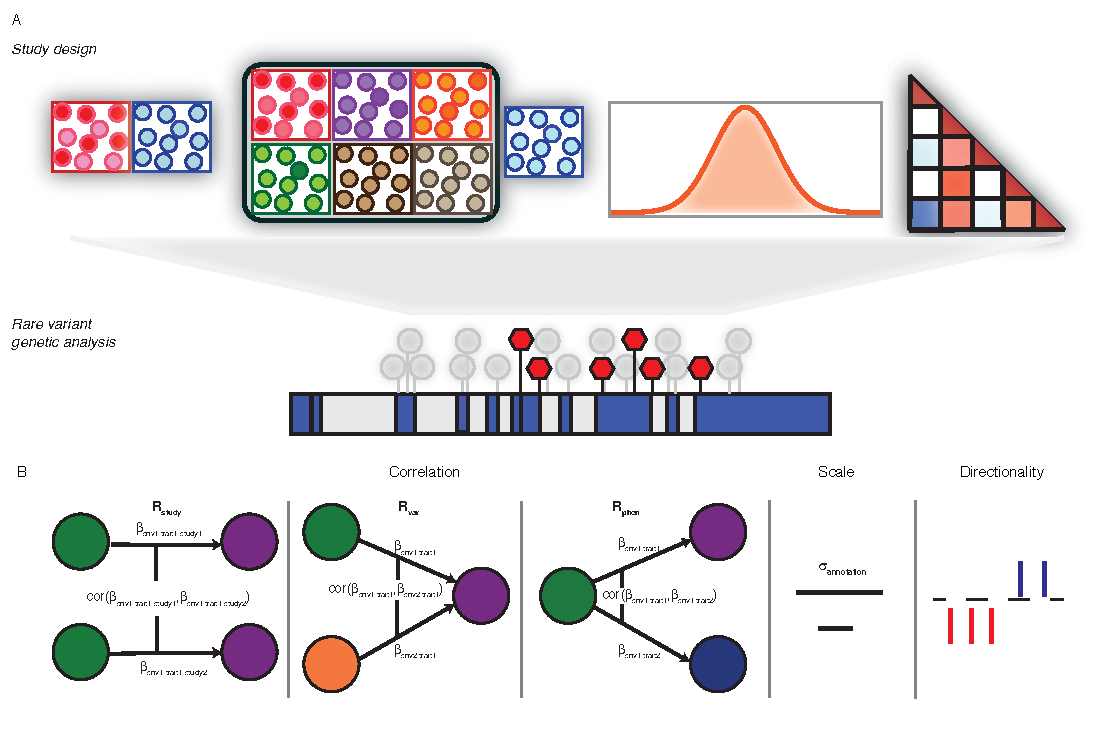
\includegraphics[width=\textwidth]{FIG1FINAL.pdf}
  \caption{Schematic overview of MRP. A. MRP is suitable for a broad range of rare variant association study designs including (from left to right): i) case-control, ii) multiple diseases with shared controls, iii) single quantitative phenotype, and iv) mixture of case-control and quantitative phenotypes. B. Diagram of factors considered in rare variant association analysis including the correlation matrices: $\mathbf{R_{\textrm{study}}}$  (expected correlation of genetic effects among a group of studies), $\mathbf{R_{\textrm{var}}}$ (expected correlation of genetic effects among a group of variants), and $\mathbf{R_{\textrm{phen}}}$ (expected correlation of genetic effects among a group of phenotypes); the scale parameter for genetic variant annotation; and the location of genetic effects, which may be used to prioritize or identify protective modifiers of disease risk.}
  \label{Fig1}
  \end{figure}
  

\section{Results}

\subsection{Methods overview}
A complete description of MRP, along with an analytical derivation, is given in the Online Methods and Appendix. Briefly, we describe the approach.

\subsubsection{Model comparison}
In Bayesian model comparison, we compare the null and alternative models via the Bayes Factor (BF) defined as the ratio of the marginal likelihoods of the observed data under two models. Here, the null model is that the effect sizes obtained across all studies for a group of variants and a group of phenotypes is zero. To complete the specification of the alternative model we consider the correlation structure, the scale, and the location of the effect sizes (which we find to be informative for alternative models where we seek to identify variants with protective effects). 

Let $N$ be the number of individuals and $K$ the number of quantitative phenotype measurements on each individual, for example, here in the applications we focus on asthma, eosinophil count, Forced Expiratory Volume in 1-second, and Forced Vital Capacity, in which case $K=4$. Let $M$ be the number of variants in a testing unit ${\bs G}$, where ${\bs G}$ can be, for example, a gene, pathway, or a network. Let $S$ be the number of studies where data is obtained from - this data may be in the form of raw genotypes and phenotypes or summary statistics including linkage-disequilibrium, effect sizes (or odds ratio), and standard error of the effect size.

In the multivariate setting we define the prior correlation structure of the effect sizes, denoted by a SMK-by-SMK matrix $\mathbf{U}$. In practice, we define $\mathbf{U}$ as a Kronecker product, an operation of matrices of arbitrary size, of three sub-matrices: an S-by-S matrix $\mathbf{R_{\textrm{study}}}$ being the correlations of genetic effects among studies where different values can be used to compare different models of association, such as for identifying heterogeneity of effect sizes between populations~\cite{band2013imputation}; an M-by-M matrix $\mathbf{R_{\textrm{var}}}$ being the correlations of genetic effects among genetic variants, which may reflect the assumption that all the PTVs in a gene may have the same biological consequence\cite{macarthur,rivas2013assessing,rivas2015effect} or prior information obtained through integration of additional data sources, such as functional assay data\cite{majithia2014rare,findlay2014saturation}, otherwise zero correlation of genetic effects may be assumed, which is used in dispersion tests like C-alpha\cite{calpha,clarke2013flexible} and SKAT\cite{skat}; and a K-by-K matrix $\mathbf{R_{\textrm{phen}}}$ being the correlations of genetic effects among phenotypes, which may be obtained from common variant data\cite{cotsapas2011pervasive,solovieff2013pleiotropy,gencorr2015}. The variance-covariance matrix of the effect sizes may be obtained from readily available summary statistic data such as in-study LD matrices, effect size estimate (or log odds ratio), and the standard error of the effect size estimate (Online Methods).

For gene discovery, the scale may be used to denote the prior spread of effect sizes. For instance, emerging empirical genetic studies have shown that within a gene protein truncating variants may have stronger effects than missense variants\cite{do2015exome}.

Thus far we have assumed that the prior mean, or location, of genetic effects is zero. This makes it feasible to analyze a large number of phenotypes without enumerating the prior mean across all phenotypes. However, in practice, we may want to proactively identify genetic variants that have effects that are consistent with a protective profile for a disease, which may exploit information from mendelian randomization studies of common variants, such as recent rare variant findings in {\it PCSK9} where truncating loss-of-function variants are found to decrease LDL and triglyceride levels, and decrease CAD risk\cite{cohen2005low,pcsk9,do2013common,cohorts2014loss}. This is straightforward to consider by including a non-zero vector as a prior mean of genetic effect (Online Methods).

Although we see advantages in adopting a Bayesian perspective, our approach could be used in a frequentist context by calculating a Bayes factor and using it as a test statistic to compute p-values (Methods, Fig.~\ref{Fig2}).
 
%\subsubsection{Mixture model for rare variant effects across multiple phenotypes}
%In Bayesian model comparison, the alternative model must be pre-specified. In practice, for gene discovery efforts, this has the attractive property that when we contrast it against a standard pre-specified null, i.e. genetic effects are zero across all studies in a group of variants and phenotypes, an analytical derivation is obtained making it computationally flexible and efficient. However, a limitation of this approach is that interpretation may not be straightforward. To make statistical inferences about the properties of the underlying mixture of genetic effects, we present a mixture model for estimating rare variant effects. Our goal is to cluster the variants into groups based on their effects on the multivariate phenotype. In particular, we allow variants to share clusters both within a gene and across the genes using a mixture model formulation of a clustering model where we also estimate the number of clusters in the data using Bayesian Information Criterion (BIC). More specifically, we can estimate (1) the proportion of non-null variants, (2) whether variants with the same annotation in one gene behave similarly, (3) whether variants across genes share effect profiles, or (4) whether different annotations differ in the magnitude of their effects.

\newpage 
%% FIGURE 2
\begin{figure}
\centering
   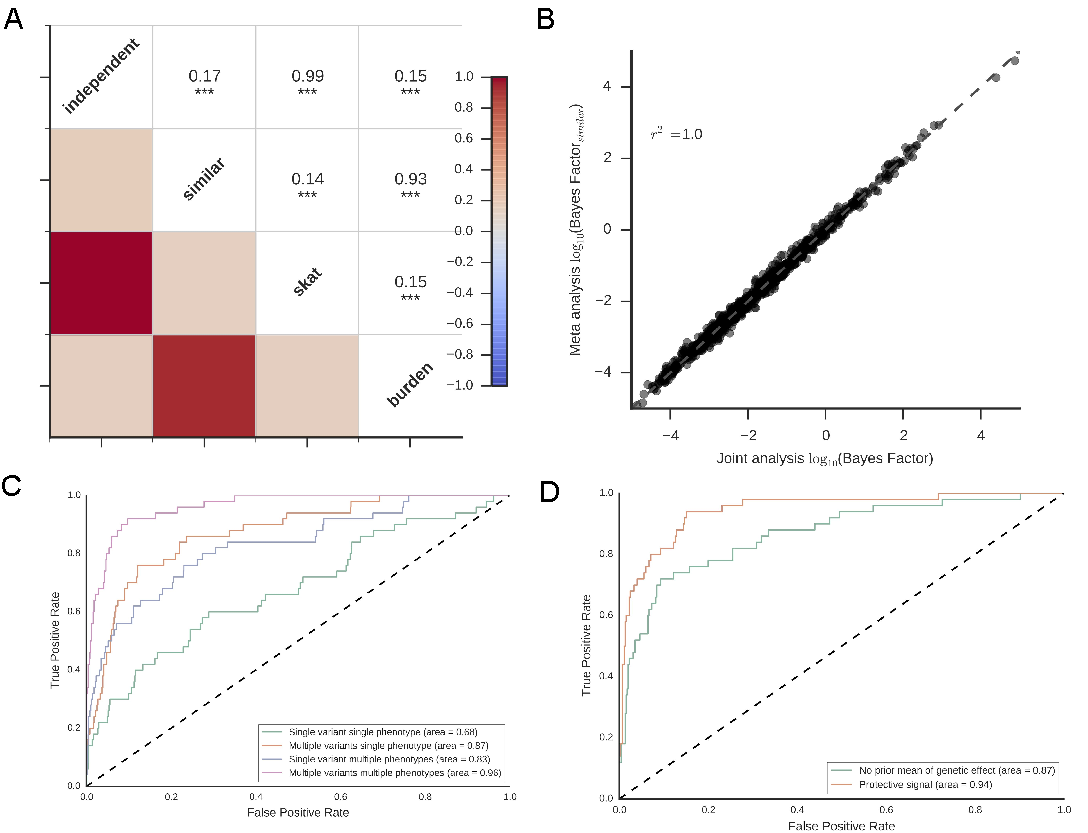
\includegraphics[width=\textwidth]{Figure2Nov2017.pdf}
  \caption{Simulation studies. A. Comparison of $-\log_{10}$(p-values) from frequentist $\textrm{BF}_{\textrm{MRP}}$ approximation for an independent effects and a similar effects model to commonly used gene-based statistical tests (skat and burden). B. Comparison of log10(Bayes Factors) obtained when raw genotype and phenotype data is available to a scenario where summary statistics only was available and similar effects across studies is assumed. C. From single variant and single phenotype to multiple variants and multiple phenotypes gene discovery: ROC curves for detecting gene association to any of the phenotypes using single variant/single phenotype association (blue) to multiple variants and multiple phenotypes association (purple). D. ROC curves for detecting gene association when incorporating prior mean of genetic effects (orange) to identify protective alleles. }
  \label{Fig2}
\end{figure}

\subsection{Simulation studies}
We first verified the analytical derivations and examined the properties of the approach under a simulation framework. 

%% Comparison to other widely used methods
\subsubsection{Comparison to frequentist gene tests}
For the analysis of multiple rare variants and a single phenotype we compared it to the burden test and the SKAT test, commonly used statistical tests in rare variant association studies of a single phenotype. We observe concordance between the frequentist methods and the Bayesian models. To compare the Bayesian models we compute p-values by using the Bayes Factor as the test statistic and approximating it using distribution properties of quadratic forms (Appendix). As expected, an independent effects model has high correlation with the gene-based test SKAT ($r^2 = 0.99$), whereas the similar effects model has high correlation with the burden test ($r^2 = 0.93$, Fig.~\ref{Fig2}A). 

\subsubsection{Summary statistic data}
To study the behavior of MRP using summary statistics we simulate two scenarios: first, the scenario where analysts have access to all the raw genotype and phenotype data; and second, the scenario where analysts only have access to summary statistics data\cite{liu2014meta}. We conducted $1000$ simulation experiments where we let $K$ (the number of phenotypes) $=3$, $M$ (the number of variants) $=10$, $S$ (the number of studies) $=2$, $N_0$ (number of individuals in study with access to all the data) $= 10000$, $N_1$ (meta-analysis study 1) $= 5000$, $N_2$ (meta-analysis study 2) $= 5000$. We find that, under the scenario where similar effects are assumed across studies, the Bayes Factors obtained using summary statistics alone are strongly correlated ($r^2 = 1$) to Bayes Factors obtained by the full genotype and phenotype data (Fig.~\ref{Fig2}B).

\subsubsection{From single variant and single phenotype analysis to multiple variants and multiple phenotypes}
To validate the flexibility of the approach we conducted a simulation experiment where we assumed an allelic architecture consistent to that discovered for {\it APOC3} in relation to coronary artery disease (CAD), triglycerides (TG), low-density lipoprotein cholesterol (LDL-C), and high-density lipoprotein cholesterol (HDL-C)\cite{apoc3,apoc32,jorgensen2014loss,cohorts2014loss}. We simulated three studies and applied the model comparison unit jointly to summary statistic data obtained for each study (Supplementary Note). Overall, we observed that considering the joint effects across multiple studies in a group of variants and phenotypes may improve ability to detect gene-based signals (Fig.~\ref{Fig2}C), and that considering prior mean of genetic effects should aid in efforts to identify protective modifiers of disease risk (Fig.~\ref{Fig2}D).

\subsection{Applications}
We demonstrate its use in rare variant analysis in the UK Biobank.

\subsubsection{Model comparison applied to asthma, eosinophil count, forced expiratory volume in 1-second, and forced vital capacity summary statistic data}
We applied the MRP model comparison approach to summary statistic data for coding variants on the UK Biobank array. The summary statistic data was generated from single variant logistic regression and linear regression analysis applied to asthma, eosinophil count, forced expiratory volume in 1-second, and forced vital capacity phenotypes. We applied the model to missense variants and PTVs for each phenotype separately (Fig.~\ref{Fig3}A-D) as well as to all phenotypes jointly (Fig.~\ref{Fig3}E) and obtained $\log_{10}$ BF for each gene. We observed evidence that missense variants and PTVs in \textit{IL33} affect eosinophil counts and offer protection from asthma from the single-phenotype analyses\cite{DeBoever179762, 10.1371/journal.pgen.1006659}, though the evidence of association was strongest for the joint analysis (Table~\ref{Tab1}). We also found evidence for associations between missense variants and PTVs in several other genes and the four phenotypes in the joint model that were not identified when considering asthma alone. For instance, \textit{GPR20}, \textit{CSF2RB}, \textit{PACS2}, and \textit{CCR3} all had $\log_{10}$ BF greater than 9 in the eosinophil count-only analysis but $\log_{10}$ BF less than 0 for the asthma-only analysis. In the joint model, the $\log_{10}$ BFs for these genes were all greater than six indicating possible associations with these traits. Besides \textit{IL33}, none of the genes with $\log_{10}$ BF greater than six in the joint model were reported in a large GWAS for allergic disease including asthma\cite{Ferreira:2017ba} though \textit{CCR3} is near a locus associated with atopy in a previous meta-analysis\cite{Ober:2011jk}. These results illustrate the ability of applying model comparison to multiple traits simultaneously to identify new genes involved in disease. 

%% FIGURE 3
\begin{figure}
\centering
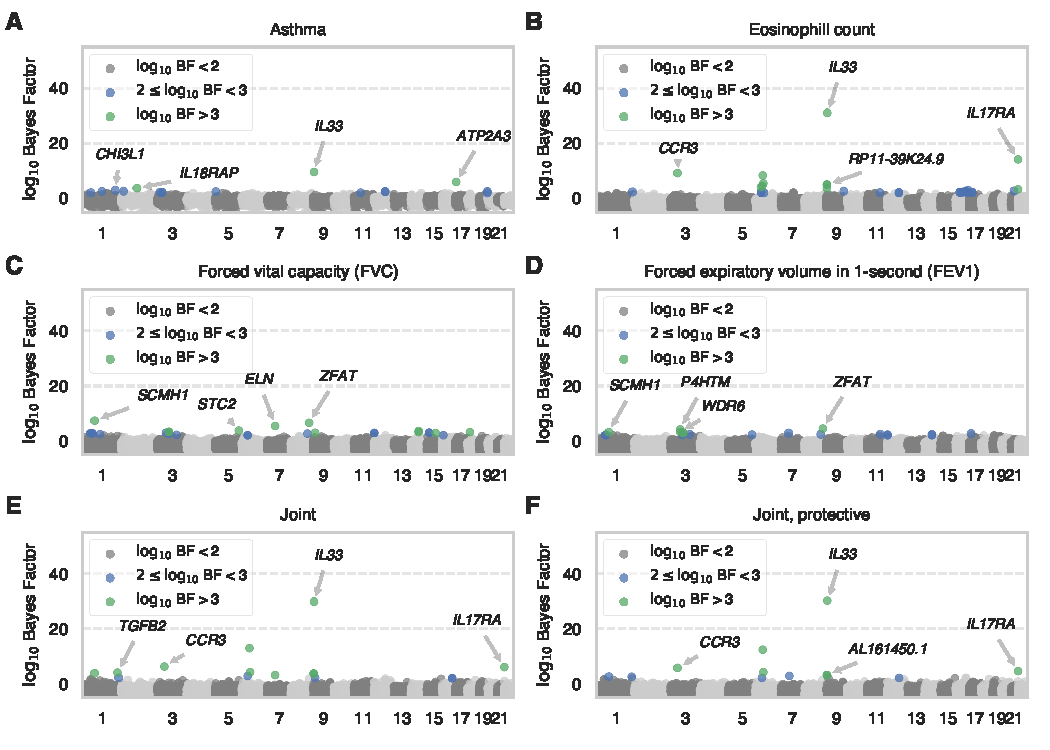
\includegraphics[width=\textwidth]{asthma_manhattan.pdf}
  \caption{$\log_{10}$ Bayes Factors from applying MRP to summary statistics for missense and protein-truncating variants from (A) eosinophil counts (INI30150), (B) forced vital capacity (FVC, INI3062), (C) forced expiratory volume in 1-second (FEV1, INI3063), (D) asthma (HC382), and (E) all four traits jointly. The four genes outside of chromosome 6 with the largest Bayes Factors are labeled in each plot. Only $\log_{10}$ Bayes Factors greater than -5 are plotted.}
  \label{Fig3}
\end{figure}

%% TABLE 3
\begin{table}
\begin{tabular}{llllll}
\toprule
{} & Joint & Eosinophil count &   FVC &  FEV1 & Asthma \\
\midrule
\textit{IL33}   &  36.6 &             31.5 &  -2.3 &  -1.9 &    9.4 \\
\textit{GPR20}  &  10.2 &             10.4 &  -0.1 &  -0.2 &        \\
\textit{ZFAT}   &  10.1 &             -3.1 &   7.8 &   5.9 &   -0.5 \\
\textit{CSF2RB} &   9.0 &              9.1 &   0.2 &  -0.1 &   -0.2 \\
\textit{SCMH1}  &   7.1 &             -1.5 &   6.8 &   2.6 &   -0.9 \\
\textit{PACS2}  &   6.2 &              9.6 &  -1.3 &  -1.6 &   -0.5 \\
\textit{CCR3}   &   6.0 &             14.0 &  -3.3 &  -3.7 &   -1.0 \\
\textit{ELN}    &   5.0 &             -1.5 &   4.9 &   2.3 &   -0.6 \\
\bottomrule
\end{tabular}
\caption{$\log_{10}$ Bayes Factors for genes outside of chromosome 6 with $\log_{10}$ Bayes Factors greater than 5 in the joint analysis.}
\label{Tab1}
\end{table}

\section{Discussion}
In this study, we developed a Bayesian model comparison approach MRP that shares information across both variants and phenotypes to identify rare variant associations. We used simulations to compare MRP to the widely used burden and SKAT tests for identifying rare variant associations and found that jointly considering both variants and phenotypes can improve the ability to detect associations. We also applied the MRP model comparison framework to summary statistic data from four traits from the UK Biobank: asthma, eosinophil counts, forced expiratory volume in 1-second (FEV1), and forced vital capacity (FVC). We identified strong evidence for the previously described association between \textit{IL33} and asthma\cite{DeBoever179762, 10.1371/journal.pgen.1006659} as well as evidence of association for several additional genes that have not been previously reported (Table~\ref{Tab1}). 

As genetic data linked to high-dimensional phenotype data continues to be made available through biobanks, health systems, and research programs, there is a large need for statistical approaches that can leverage information across different genetic variants, phenotypes, and studies to make strong inferences about disease-associated genes. The approach presented here relies only on summary statistics from marginal association analyses which can be shared with less privacy concerns compared to raw genotype and phenotype data. Combining joint analysis of variants and phenotypes with meta-analysis across studies offers new opportunities to identify gene-disease associations.

\newpage
\section{Methods}
 
\subsection{MRP model comparison for association testing}
We consider the multivariate linear regression model 
$$\underset{\left(N\times K\right)}{\mathbf{\textrm{Y}}} 
= \underset{\left(N\times K\right)}{\mathbf{\Psi}}  + \underset{\left(N\times M\right)}{\mathbf{\textrm{X}}}\underset{\left(M \times K\right)}{\mathbf{\textrm{B}}} 
+ \underset{\left(N\times K\right)}{\mathbf{\textrm{E}}},$$
where the matrices $\mathbf{\textrm{Y}} = \left[{y}_{i k}\right]$, $\mathbf{\textrm{X}} = \left[ x_{i m}\right]$, 
$\mathbf{\textrm{B}} = \left[ \beta_{m k} \right]$ and $\mathbf{\textrm{E}} = \left[e_{i k}\right]$  describe the phenotype values ($y_{i k}$),
copies of minor allele ($x_{i m}$), variant-phenotype effects ($\beta_{m k}$), and residual errors ($e_{i k}$), 
for individual $i$, phenotype $k$, and variant $m$. 
We assume that each phenotype has been transformed to a standard normal
distribution and that the columns of ${\mathbf{{\textrm{X}}}}$ 
have been centered, which means that the estimate for the intercept term ${\mathbf{\Psi}}$ is 0 and independent of the estimate of ${\mathbf{\textrm{B}}}$.
We use vectorized notation where the rows of ${\mathbf{\textrm{B}}}$ form vector 
$\bs {{ \beta}} = \left(\bs {{ \beta}}_{1},\dots,\bs {{\beta}}_{M}\right)^{\intercal}$
of length $MK$.

\noindent We define the MRP model comparison as a Bayes factor (BF) between the alternative model, where at least one variant
affects at least one phenotype, and the null model, where all variant-phenotype effects are zero.  
\noindent BF is the ratio of the marginal likelihoods for these two models: 
$$ \textrm{BF} = \frac{\int_{{\bs {\beta}}}p\left(\mathbf{\textrm{Data}}|{\bs {\beta}}\right)p\left({\bs {\beta}}|\textrm{ALT}\right)d{\bs {\beta}}}{\int_{{\bs {\beta}}}p\left(\mathbf{\textrm{Data}}|{\bs {\beta}}\right)p\left({\bs {\beta}}|\textrm{NULL}\right)d{\bs {\beta}}},$$ 
where Data can correspond either to the effect size estimates $\bs {\widehat{ \beta}}$ and the estimated variance-covariance matrix of  $\bs {\widehat{ \beta}}$, $\widehat{\mathbf{\textrm{V}}}_{\bs{\beta}}$, or to the original phenotypes and genotypes, 
$\underset{\left(N\times K\right)}{\mathbf{\textrm{\textrm{Y}}}}$ and $ \underset{\left(N\times M\right)}{\mathbf{\textrm{\textrm{X}}}}$, and any other covariates that we
want to regress out from the phenotypes. 

The prior distribution for the null model, $p\left({\bs {\beta}}|\textrm{NULL}\right)$, is simply the point mass at $\bs \beta = 0$.
In subsection~\ref{approxlikelihood} we show how we approximate the likelihood function for $\bs \beta$, $p\left(\mathbf{\textrm{Data}} | {\bs {\beta}}\right)$,
in subsection~\ref{prioralt} we define the prior distribution $p\left({\bs {\beta}}|\textrm{ALT}\right)$ for the alternative model, 
and finally, in subsection~\ref{bfmodel}, we compute the BF.

\subsubsection{Likelihood function} 
\label{approxlikelihood}
\noindent A maximum likelihood estimator of $\mathbf{\textrm{B}}$ is given by the ordinary least-squares method
$$\widehat{\mathbf{\textrm{B}}} = \left(\mathbf{\textrm{X}}^\intercal\mathbf{\textrm{X}}\right)^{-1}\mathbf{\textrm{X}}^{\intercal}\mathbf{\textrm{Y}},$$
that in vectorized form is denoted by   
$\bs {\widehat{ \beta}} = \left(\bs {\widehat{ \beta}}_{1},\dots,\bs {\widehat{\beta}}_{M}\right)^{\intercal}.$
An estimator of the variance-covariance of $\widehat{\bs \beta}$  is given by 
$$\widehat{\textrm{V}}_{\mathbf{\bs \beta}} =  \left(\mathbf{\textrm{X}}^\intercal\mathbf{\textrm{X}}\right)^{-1}\otimes \widehat{\textrm{V}}_{\mathbf{\textrm{Y}}},$$
where $\widehat{\textrm{V}}_{\mathbf{\textrm{Y}}}$ is the estimated residual variance-covariance matrix of $\mathbf{\textrm{Y}}$ given $\mathbf{\textrm{X}}$. 

\noindent 
%Let $\bs {\widehat{ \beta}} = \left(\bs {\widehat{ \beta}}^{\intercal}_{1},\dots,\bs {\widehat{\beta}}^{\intercal}_{m}\right)^{\intercal}$ be a vector of point estimates of all $MK$ effects. 
Following Band et al.\cite{band2013imputation}, we approximate the likelihood function of $\bs {\beta}$ by a multivariate normal distribution with mean $\bs {\widehat{\beta}}$ and variance-covariance matrix $\widehat{\textrm{V}}_{\bs {\beta}}$. Note that by approximating $\Vy$ by the trait correlation matrix, this likelihood approximation does not require access to the individual level data $\mathbf{\textrm{X}}$ and $\mathbf{\textrm{Y}}$ but only to the 
summary data of effect sizes $\bs {\widehat{\beta}}$, LD-matrix $\mathbf{\textrm{X}}^\intercal\mathbf{\textrm{X}}$ and a trait correlation estimate.


\subsubsection{Prior of $\bs{\beta}$ in the alternative model} 
\label{prioralt}
\noindent We construct the prior distribution $p\left({\bs {\beta}} | \textrm{ALT} \right)$ for the alternative model in three steps allowing 
user to specify correlations between effects of different variants on different traits across different studies.

\noindent In a single study, the prior density for ${\bs {\beta}}$ incorporates the expected correlation of genetic effects among 
a group of variants ($\mathbf{R}_{\textrm{var}}$) and among a group of phenotypes ($\mathbf{R}_{\textrm{phen}}$). 
In addition, we  incorporate an expected spread of the effect size of each variant by scaling $\mathbf{R}_{\textrm{var}}$ as 
$$\mathbf{S}_{\textrm{var}} = \Delta\left(\sigma_m\right) \mathbf{R}_{\textrm{var}} \Delta\left(\sigma_m\right),$$
\noindent where $\Delta\left(\sigma_m\right)$ is a diagonal matrix with entries $\sigma_m$ determining the spread of the effect size distribution for each variant $m \leq M$. Thus, we can model settings where, e.g., protein-truncating variants have larger effect sizes ($\sigma = 1$) than missense variants ($\sigma = 0.1$). 
Note that when $\sigma_m = 1$ for all $m$ then $\mathbf{S}_{\textrm{var}} = \mathbf{R}_{\textrm{var}}$. 
\noindent All in all, our prior density for ${\bs \beta}$ under alternative model is 
$${\bs {\beta}}|\textrm{ALT} \sim \mathcal{N}\left(\mathbf{0}, \mathbf{U}\right), \textrm{ where } \mathbf{U} = \mathbf{S}_{\textrm{var}} \otimes \mathbf{R}_{\textrm{phen}}.$$

\noindent When we have data from multiple studies 
we allow for possible differences in genetic effects across ethnicities or populations 
extending the Approximate Bayes Factors of Band et al.~\cite{band2013imputation}
and the summary statistics approach of RAREMETAL ~\cite{liu2014meta} from univariate to multivariate phenotypes.
Let $\bs {\widehat{ \beta}} = \left(\widehat{ \beta}_{s,m,k}\right)=\left(\widehat{\beta}_{1,1,1}, \widehat{\beta}_{1,1,2}, \dots, \widehat{\beta}_{1,1,K}, \widehat{\beta}_{1,2,1}, \dots, \widehat{\beta}_{1,2,K}, \dots, \widehat{\beta}_{1,M,K}, \widehat{\beta}_{2,1,1}, \dots, \widehat{\beta}_{S,M,K}\right),$ where $S$ is the number of studies, $M$ is the number of variants, and $K$ is the number of phenotypes. 
As with a single study, we incorporate the expected correlation of genetic effects between a pair of variants and a single phenotype using the matrix $\mathbf{S_{\textrm{var}}}$, between a variant and a pair of phenotypes using the matrix $\mathbf{R_{\textrm{phen}}}$, and we introduce the matrix $\mathbf{R_{\textrm{study}}}$ to specify prior on the similarity in effect sizes across the studies.
Thus, the prior is
$${\bs {\beta}} \sim \mathcal{N}\left(\mathbf{0}, \mathbf{U}\right), \textrm{ where } 
\mathbf{U} = \mathbf{R}_{\textrm{study}}\otimes\left(\mathbf{S}_{\textrm{var}} \otimes \mathbf{R}_{\textrm{phen}}\right).$$

\noindent It is straightforward to include a non-zero vector ${\bs\mu}$ as a prior mean of genetic effects, in which case the prior is
$${\bs {\beta}} \sim \mathcal{N}\left({\bs \mu},\mathbf{U}\right).$$
We use this, for example, when screening for protective rare variants that have a pre-specified beneficial profile on a set of risk factors.


\subsubsection{$\textrm{BF}_{\textrm{MRP}}$} 
\label{bfmodel}
\noindent The Bayes Factor is the ratio of the marginal likelihoods between the alternative and the null model. 
\noindent The marginal likelihood for the alternative model is 
$$ \int_{{\bs {\beta}}} p\left(\mathbf{\textrm{Data}}|{\bs {\beta}}\right) p\left({\bs {\beta}}|\textrm{ALT}\right)d{\bs {\beta}} = c \times \mathcal{N}\left({ {\widehat{\bs \beta}}}; {\bs \mu},  \widehat{\mathbf{\textrm{V}}}_{{\bs {\beta}}} + \mathbf{U}\right)$$
\noindent and the marginal likelihood for the null model is 
$$\int_{{\bs {\beta}}} p\left(\mathbf{\textrm{Data}}|{\bs {\beta}}\right) p\left({\bs {\beta}}|\textrm{NULL}\right)d{\bs {\beta}} = c \times \mathcal{N}\left({ {\widehat{\bs \beta}}}; 0,  \widehat{\mathbf{\textrm{V}}}_{{\bs {\beta}}}\right).$$
\noindent In Appendix (\ref{app1}) we show how we compute the Bayes Factor
$$\textrm{BF}_{\textrm{MRP}} = \frac{\det\left(\widehat{\mathbf{\textrm{V}}}_{{\bs {\beta}}} + \mathbf{U} \right)^{-\frac{1}{2}}
\exp\left[-\frac{1}{2}\left({\bs {\widehat{\beta}} - {\bs \mu}}\right)^{\intercal}\left(\widehat{\mathbf{\textrm{V}}}_{{\bs {\beta}}} + \mathbf{U}\right)^{-1}\left({\bs {\widehat{\beta}}} - {\bs \mu}\right)\right]}
{\det \left( \widehat{\mathbf{\textrm{V}}}_{\bs {\beta}}\right)^{-\frac{1}{2}}\exp \left[-\frac{1}{2}{\bs {\widehat{\beta}}}^{\intercal}\, \widehat{\mathbf{\textrm{V}}}_{\bs {\beta}}^{-1} 
\,{\bs {\widehat{\beta}}}\right]}.$$


When $\bs \mu=0$, $\textrm{BF}_{\textrm{MRP}}$ is an increasing function of the following quadratic form
\begin{equation}\label{quadratic_form}
Q(\bs{\widehat{\beta}};\widehat{\mathbf{\textrm{V}}}_{{\bs {\beta}}},\mathbf{U})=
\bs{\widehat{\beta}^\intercal} \left(\widehat{\mathbf{\textrm{V}}}_{{\bs {\beta}}}^{-1} - (\widehat{\mathbf{\textrm{V}}}_{{\bs {\beta}}}+\mathbf{U})^{-1}\right) \bs{\widehat{\beta}}.
\end{equation}
Furthermore, this quadratic form is the only part of the $\textrm{BF}_{\textrm{MRP}}$ that depends on $\bs {\widehat{\beta}}$.
Thus, by deriving a distribution of $Q(\bs{\widehat{\beta}};\widehat{\mathbf{\textrm{V}}}_{{\bs {\beta}}},\mathbf{U})$
under the null model we can compute a p-value when $\textrm{BF}_{\textrm{MRP}}$ is used as a test statistic.
According to basic properties of quadratic forms of Gaussian variables,
$Q(\bs{\widehat{\beta}};\widehat{\mathbf{\textrm{V}}}_{{\bs {\beta}}},\mathbf{U}) \sim \sum_{i=1}^n d_i \chi^2_i$, where $\chi_i^2$
are an independent sample from $\chi_1^2$ distribution (chi-square with one degree of freedom),
and $d_i$ are the eigenvalues of matrix
$I-(\widehat{\mathbf{\textrm{V}}}_{{\bs {\beta}}}+\mathbf{U})^{-1}\, \widehat{\mathbf{\textrm{V}}}_{{\bs {\beta}}}$.
The distribution function for a mixture of chi-squares can be numerically evaluated by
the R-package `CompQuadForm'~\cite{Duchesne2010}.

\subsection{UK Biobank Data}
\subsubsection{GWAS Summary Statistics}
We performed genome-wide�association analysis using PLINK v2.00a(17 July 2017) as previously described~\cite{DeBoever179762}. For asthma, we used the Firth-fallback in PLINK, a hybrid algorithm which normally uses the logistic regression code described in�(Hill 2017), but switches to a port of logistf() (https://cran.r-project.org/web/packages/logistf/index.html) in two cases: (1) one of the cells in the 2x2 allele count by case/control status contingency table is empty (2) logistic regression was attempted since all the contingency table cells were nonzero, but it failed to converge within the usual number of steps. We used the following covariates in our analysis: age, sex, array type, and the first four principal components, where array type is a binary variable that represents whether an individual was genotyped with UK Biobank Axiom Array or UK BiLEVE Axiom Array. For variants that were specific to one array, we did not use array as a covariate. Asthma cases were defined using both Hospital Episode Statistics and verbal questionnaire responses. We used the provided values from the UK Biobank for eosinophil counts, forced vital capacity (FVC), and forced expiratory volume in 1-second (FEV1). The phenotype codes used throughout (asthma=HC382, eosinophil count=INI30150, Forced Expiratory Volume in 1-second (FEV1)=INI3063, and Forced Vital Capacity (FVC)=INI3062) correspond to the phenotype codes used in on the Global Biobank Engine [\url{https://biobankengine.stanford.edu}].

\subsubsection{Genetic Correlations}
We calculated the genetic between asthma, eosinophil counts, forced vital capacity (FVC), and forced expiratory volume in 1-second (FEV1) using the MultiVariate Polygenic Mixture Model (MVPMM)~\cite{DeBoever2017}. Briefly, MVPMM estimates genetic correlation given GWAS summary statistics (effect size and standard error of effect size estimate) by modeling GWAS summary statistics as generated from one of two mixture components. Summary statistics from variants in the null component are modeled as being drawn from a multivariate normal distribution with zero mean and covariance matrix that captures correlation in the summary statistics due to the use of shared subjects or other sources of correlation. Summary statistics from variants in the non-null component are modeled as being drawn from a multivariate normal distribution with zero mean, but the covariance matrix for the non-null component combines the covariance matrix from the null component with another covariance matrix that captures the genetic correlation between the phenotypes being considered.

\subsubsection{UK Biobank Asthma Application}
For the Manhattan plots \ref{Fig3} and table \ref{Tab1}, we removed any genes with non-unique gene symbols. We also removed the sense overlapping gene \textit{CTD-3064M3.3} and and the antisense gene \textit{ZFAT-AS1} since these genes overlap \textit{GPR20} and \textit{ZFAT} respectively and therefore have the same $\log_{10}$ Bayes Factors as those genes.

%%%
%
%\subsection{MRP mixture modeling for effect size estimation} 
%\label{mrpmm}
%Index genes by $j = 1,\dots, J$ and denote variant $m$ in gene $j$ by $v_{jm}$. Our goal is to cluster the variants into groups based on their effects on the multivariate phenotype. To compare models with different numbers of clusters we use the Bayesian Information Criterion (BIC).  
%
%We represent each cluster $c$ by a mean effect size 
%$$ \bs b_c \sim \mathcal{N}\left(0,\bs \Theta_0\right),$$
%where $\bs \Theta_0$ is our prior estimate of genetic correlation across the traits; 
%and a covariance structure
%$\bs \Sigma_c = \widehat{\mathbf{\textrm{V}}}_Y $ (when phenotype data available) or $\bs \Sigma_c = \widehat{\mathbf{\textrm{V}}}_{jm}$ (when only summary statistics available),  
%where $\widehat{\mathbf{\textrm{V}}}_Y$ is an estimate of the phenotype correlation and remains fixed across the clusters, and $\widehat{\mathbf{\textrm{V}}}_{jm}$ will be defined below. 
%(Extensions to cluster-specific $\bs \Sigma_c$ are possible but not considered in this work.)
%
%Consider the model with $C>1$ clusters. To model the sharing of clusters across the genes we first draw a $C$ dimensional probability vector 
%$$\bs \pi_{0} \sim \mathrm{Dirichlet}\left(1,1,1,\ldots ,1\right).$$ Next, for each gene $j$, we draw a probability vector 
%$$\bs \pi_{j} | \bs \pi_{0} \sim \mathrm{Dirichlet}\left(\alpha \bs \pi_{0}\right)$$
%to determine the mixture proportions $\pi_{jc}$ that tell how the variants in gene $j$ are distributed across the clusters $c$. The parameter $\alpha$ governs how much sharing of clusters exists across genes with prior 
%$$\alpha \sim \textrm{Inv-Gamma}\left(1,1\right).$$ 
%To relate the clusters to the observed data, the phenotype of
%individual $i$ with a rare allele of variant $m$ with annotation $a$ in gene $j$ is
%
%$$\bs y_{i} | \left( \bs \pi_j, {\bs b}, \sigma_a \right) \sim \sum_{c=1}^{C}\pi_{jc}\mathcal{N}\left(\sigma_{a} \bs b_c, \bs \Sigma_c\right) $$
%where $\sigma_a$ corresponds to a scale parameter for annotation $a$ across all the clusters, where annotations may be, e.g., 
%protein truncating variant (PTV), missense variant, or other functional annotation category, with an inverse-gamma prior
%$$\sigma^2_{a} \sim \textrm{Inv-Gamma}\left(sh_a, sc_a\right),$$
%with hyperparameter values $sh_a$ (shape) and $sc_a$ (scale).
%At the above formulation, we assume that each individual carriers at most one of the rare variants considered.
%
%If we have access only to summary statistics of estimated effect sizes 
%$\widehat{\bs \beta}_{jm}$ and estimated variance-covariance 
%matrices $\widehat{\mathbf{\textrm{V}}}_{jm}$ for each variant $m$ in gene $j$, our sampling model for the data is
%$$\widehat{\bs \beta}_{jm} | \left( \bs \pi_j, {\bs b}, \sigma_a \right) \sim \sum_{c=1}^{C}\pi_{jc}\mathcal{N}\left(\sigma_{a} \bs b_c, \widehat{\mathbf{\textrm{V}}}_{jm} \right).$$
%Similar to the individual level data model above, this formulation assumes independence between the variants, which is 
%approximately true when each individual carries at most one of the rare variants considered.
%A connection between the two data types is
%that $\widehat{\bs \beta}_{jm} \approx \frac{1}{1-2f_{jm}} \overline{\bs y}_{jm}$ and
%$\widehat{\mathbf{\textrm{V}}}_{jm} \approx \frac{1}{2 N f_{v_{jm}}(1-2f_{jm})} \widehat{\mathbf{\textrm{V}}}_{Y}$ where $f_{jm}$ is the frequency of the 
%rare allele at variant $m$ of gene $j$ among the $2N$ haplotypes 
%and $\overline{\bs y}_{jm}$ is the mean phenotype of the carrier individuals of that allele.
%
%In the Appendix (\ref{app2}) we give an algorithm to analyze this mixture model using summary statistic data.
%
%To compare the models with different numbers of clusters we use BIC\cite{schwarz1978estimating}, defined for the model $\mathcal{M}_C$ with $C$ clusters, as
%$$BIC_C = -2\log\left(p\left(D | \widehat{\theta_C}, \mathcal{M}_C\right)\right) + \nu_C \log\left(n\right)$$ where $D$ denotes the observed data, $\widehat{\theta_C}$ is the vector of maximum likelihood estimates of the parameters of $\mathcal{M}_C$, $\nu_c$ is the number of independent parameters of $\mathcal{M}_c$ and $n$ is the number of data points. The difference in BIC values between two models approximates twice the logarithm of the Bayes factor between the models.
%
%In the Appendix (\ref{app2}) we give an algorithm to analyze this mixture model using summary statistic data.

\subsection{Author Contributions}
M.A.R. and M.P. designed the method and derived all analytical calculations. M.A.R., M.P., and C.D. wrote the manuscript. Y.T., M.A., and C.D. provided analysis and designed figures. T.P. designed hDF5 tables and implementation of loaders. M.J.D. provided critical feedback on methodology.

\subsection{Acknowledgments}
This research has been conducted using the UK Biobank Resource under Application Number 24983. We thank all the participants in the UK Biobank study. M.A.R. and C.D. are supported by Stanford University and a National Institute of Health center for Multi- and Trans-ethnic Mapping of Mendelian and Complex Diseases grant (5U01 HG009080). C.D. is supported by a postdoctoral fellowship from the Stanford Center for Computational, Evolutionary, and Human Genomics and the Stanford ChEM-H Institute. Y .T. is supported by Funai Overseas Scholarship from Funai Foundation for Information Technology and the Stanford University Biomedical Informatics Training Program. The primary and processed data used to generate the analyses presented here are available in the UK Biobank access management system (https://amsportal.ukbiobank.ac.uk/) for application 24983, ?Generating effective therapeutic hypotheses from genomic and hospital linkage data? (http://www.ukbiobank.ac.uk/wp-content/uploads/2017/06/24983-Dr-Manuel-Rivas.pdf), and the results are displayed in the Global Biobank Engine (https://biobankengine.stanford.edu). We would like to thank the Customer Solutions Team from Paradigm4 who helped us implement efficient databases for queries and application of inference methods to the data, and also implemented optimized versions of truncated singular value decomposition. M.A.R. is a paid consultant in Genomics PLC.

\section{Appendix}
\subsection{MRP Bayes Factor computation} \label{app1}
To compute the Bayes Factor 
$$\textrm{BF}_{\textrm{MRP}} = \frac{\det\left(\widehat{\mathbf{\textrm{V}}}_{{\bs {\beta}}} + \mathbf{U} \right)^{-\frac{1}{2}}
\exp\left[-\frac{1}{2}\left({\bs {\widehat{\beta}} - {\bs \mu}}\right)^{\intercal}\left(\widehat{\mathbf{\textrm{V}}}_{{\bs {\beta}}} + \mathbf{U}\right)^{-1}\left({\bs {\widehat{\beta}}} - {\bs \mu}\right)\right]}
{\det \left( \widehat{\mathbf{\textrm{V}}}_{\bs {\beta}}\right)^{-\frac{1}{2}}\exp \left[-\frac{1}{2}{\bs {\widehat{\beta}}}^{\intercal}\, \widehat{\mathbf{\textrm{V}}}_{\bs {\beta}}^{-1} 
\,{\bs {\widehat{\beta}}}\right]},$$
we first consider the term inside the exponential function:
$$ \mathcal{E} \left(\widehat{\bs \beta}, \bs \mu, \widehat{\mathbf{\textrm{V}}}_{\bs {\beta}}, \mathbf{U}\right) = 
\frac{1}{2}\, {\bs {\widehat{\beta}}}^{\intercal}\, \widehat{\mathbf{\textrm{V}}}_{\bs {\beta}}^{-1} \,{\bs {\widehat{\beta}}}
-\frac{1}{2}\left({\bs {\widehat{\beta}} - {\bs \mu}}\right)^{\intercal}\left(\widehat{\mathbf{\textrm{V}}}_{{\bs {\beta}}} + \mathbf{U}\right)^{-1}\left({\bs {\widehat{\beta}}} - {\bs \mu}\right).
$$
Since $\widehat{\mathbf{\textrm{V}}}_{\bs {\beta}}$ and $\mathbf{U}$ are typically defined through Kronecker products of smaller matrices, their inverses
are easier to compute than the inverse of their sum. Hence we use Woodbury matrix identity to write
$$ 
\mathcal{E} \left(\widehat{\bs \beta}, \bs \mu, \widehat{\mathbf{\textrm{V}}}_{\bs {\beta}}, \mathbf{U}\right) = 
\frac{1}{2}\, {\bs {\widehat{\beta}}}^{\intercal}\, \widehat{\mathbf{\textrm{V}}}_{\bs {\beta}}^{-1} \,{\bs {\widehat{\beta}}}
-\frac{1}{2}\left({\bs {\widehat{\beta}} - {\bs \mu}}\right)^{\intercal} \left( \widehat{\mathbf{\textrm{V}}}_{\bs {\beta}}^{-1} - \widehat{\mathbf{\textrm{V}}}_{\bs {\beta}}^{-1} 
\left(\mathbf{U}^{-1} + \widehat{\mathbf{\textrm{V}}}_{\bs {\beta}}^{-1} \right)^{-1} \widehat{\mathbf{\textrm{V}}}_{\bs {\beta}}^{-1} \right ) 
\left({\bs {\widehat{\beta}} - {\bs \mu}}\right).
$$

To simplify the determinant calculation we write 
$$\det\left( \widehat{\mathbf{\textrm{V}}}_{{\bs {\beta}}} + \mathbf{U} \right) = \det\left( \widehat{\mathbf{\textrm{V}}}_{{\bs {\beta}}}\right) \det\left( \mathbf{I} + \widehat{\mathbf{\textrm{V}}}_{{\bs {\beta}}}^{-1} \mathbf{U}\right).$$
The logarithm of the Bayes Factor is then
$$\log \left( \textrm{BF}_{\textrm{MRP}} \right) = 
-\frac{1}{2} \log \left( \det\left( \mathbf{I} + \widehat{\mathbf{\textrm{V}}}_{{\bs {\beta}}}^{-1} \mathbf{U} \right) \right)  + \mathcal{E} \left(\widehat{\bs \beta}, \bs \mu, \widehat{\mathbf{\textrm{V}}}_{\bs {\beta}}, \mathbf{U}\right).$$


If studies do not share individuals, $\widehat{\mathbf{\textrm{V}}}_{{\bs {\beta}}}$ is a block-diagonal matrix 
$$\widehat{\mathbf{\textrm{V}}}_{{\bs {\beta}}}=
 \left[\begin{array}{c|c|c|c}
 \widehat{\mathbf{\textrm{V}}}^{1}_{{\bs \beta}} & 0 & \cdots &0\\ \hline
0 & \widehat{\mathbf{\textrm{V}}}^{2}_{{\bs \beta}}&\cdots &0 \\ \hline
\vdots & &\ddots &\vdots \\ \hline
0 & 0 &\cdots & \widehat{\mathbf{\textrm{V}}}^{S}_{{\bs {\beta}}}\\
\end{array}\right].$$
If studies share individuals, e.g., controls, 
we take the approach of Cichonska et al.~\cite{cichonska2016metacca} to use summary level data
to estimate the correlation structure of the non-diagonal blocks caused by overlapping individuals. 


%\subsection{MRP Mixture model computation} \label{app2}
%For multiparameter models, the joint posterior distribution may be difficult to sample from directly. 
%Often, it is easier to sample sequentially from the full conditional distribution of each parameter~\cite{hoff2009first} using a 
%Gibbs sampler, a Markov Chain Monte Carlo (MCMC) algorithm, that constructs a dependent sequence of parameter 
%values whose distribution approximates the joint posterior distribution~\cite{geman1984stochastic,casella1992explaining,hoff2009first}. 
%We propose the following algorithm that is augmented by a Metropolis-Hastings step to update the annotation scaling parameters $\bs \sigma_a^2$ and the sharing intensity parameter $\alpha$. 
%
%%% 03.01.2016 
%The implementation of the Gibbs sampler requires the following data structure: 
%Within gene $j$, the variants $1,\ldots,M_j$ are assigned to clusters $c=1,...,C$,
%each of which is represented by a parameter $(\bs b_c, \bs \Sigma_c)$ as described in Section~\ref{mrpmm} with
%$\bs \Sigma_c = \Vy$ being fixed to an estimate of the trait covariance across the clusters or $\widehat{\mathbf{\textrm{V}}}_{jm}$ for each allele when using summary statistics.
%
%The Gibbs sampler is run for $n_{\text{burn}} + n_{\text{iter}}$ iterations, of which the first $n_{\text{burn}}$
%are discarded as an initial "burn-in" part. 
%With the prior distributions given in Section~\ref{mrpmm}, and superscripts in parentheses denoting iteration, the algorithm is as follows:
%
%\begin{enumerate}
%\item Initialize 
%	\begin{enumerate}
%	\item Draw $\alpha^{\left(0\right)} \sim \textrm{Inv-Gamma}\left(1,1\right);$
%	\item Draw $\bs \pi_0^{\left(0\right)} \sim \textrm{Dirichlet}\left(1,1,1,\ldots, 1\right);$ %OK
%	\item Draw for each gene $j$: $\bs \pi_j^{\left(0\right)} \sim \textrm{Dirichlet}\left(\alpha^{(0)} \bs \pi_0^{\left(0\right)} \right);$
%	\item ${\bs b}^{\left(0\right)}_{1} = \bs 0;$
%	\item For each $c$ in $2,\dots,C$ draw $\bs b_c^{\left(0\right)} \sim \mathcal{N}\left(\bs 0, \bs \Theta_0\right);$
%	\item $\left(\sigma^2_{a}\right)^{\left(0\right)} = 0.2^2$ for all $a$.  
%	\end{enumerate}
%
%	\item Repeat for iteration $t = 1, 2, \dots, n_{\text{burn}} + n_{\text{iter}}$
%	\begin{enumerate}
%	\item Update $\bs \pi_0$. We use a Metropolis-Hastings sub-step~\cite{hastings1970monte} using a proposal centred around the current value. 
%	We sample a proposal value for 
%	$$\bs \pi_0^{'} \sim \textrm{Dirichlet}\left(\gamma \bs \pi_0^{(t-1)} \right).$$ 
%	To calculate the acceptance probability, we define the normalizing constant for the C-dimensional Dirichlet distribution with parameters $\bs z$ as
%	$$ D(\bs z) = \frac{\Gamma \left( \sum_{c=1}^C z_c \right) }{\prod_{c=1}^C \Gamma\left ( z_c \right)}$$ and the density at point $\bs x$ as
%	$$p_{\textit Dir}(\bs x | \bs z ) = D(\bs z) \prod_{c=1}^C x_c^{ z_c -1}.$$
%	With this notation the Metropolis-Hastings transition probability from $\bs \pi_0^{(t-1)}$ to $\bs \pi_0^{'}$ is $p_{\textit Dir}\left (\bs \pi_0^{'} | \gamma \bs \pi_0^{(t-1)} \right)$
%	and the density of the observed data depends on $\bs \pi_0^{(t-1)}$ only through the product $\prod_{j=1}^J p_{\textit Dir}\left (\bs \pi_j | \alpha \bs \pi_0^{(t-1)} \right ).$
%	Hence, the acceptance probability of the proposal is
%	$$
%	\lambda = \min\left( 1, \frac{  p_{\textit Dir}\left (\bs \pi_0^{(t-1)} | \gamma \bs \pi_0^{'} \right ) \prod_{j=1}^J p_{\textit Dir}\left (\bs \pi_j | \alpha \bs \pi_0^{'} \right )  }
%	{p_{\textit Dir}\left (\bs \pi_0^{'} | \gamma \bs \pi_0^{(t-1)} \right ) \prod_{j=1}^J p_{\textit Dir}\left (\bs \pi_j | \alpha \bs \pi_0^{(t-1)} \right ) } \right)$$
% Thus, with probability $\lambda$, we set $\bs \pi^{\left(t \right)}_0 = \bs \pi^{'}_0$ and with probability $1-\lambda$ we set $\bs \pi^{\left(t \right)}_0 = \bs \pi^{(t-1)}_0$.
%	
%	\item For each gene $j=1,\ldots , J$ update $\bs \pi_j$: $$\bs \pi_j \sim \textrm{Dirichlet}\left(\alpha \bs \pi_0 + \left(\sum_{m=1}^{M_j}\delta_{jm} = 1, 
%	\sum_{m=1}^{M_j}\delta_{jm} = 2, \dots, \sum_{m=1}^{M_j} \delta_{jm} = C\right)\right),$$
%	where $\delta_{jm}$ is the index of the cluster to which the variant $m$ of gene $j$ belongs to.
%	
%	%% update cluster membership 
%	\item Update $\delta_{jm}$ for all $j=1,\ldots, J$ and $m=1,\ldots,M_j$. 
%	For all $c$ compute $$p^'_{jmc} = p\left(\hat{\bs \beta}_{jm}; \bs b_c, \bs \Sigma_c\right)\pi_{jc},$$
%	and renormalize in such a way that $p_{jmc} \propto p^'_{jmc}$ sums to 1 over $c$.
%	Then we sample $$\delta_{jm} \sim \textrm{Discrete} (p_{jmc}).$$
%		
%	%% update cluster effect profile
%	\item Update $\bs b_{c}$ using a Gibbs update (see derivation below) from a Gaussian distribution with
%	\begin{eqnarray*}	
%	\textrm{mean}&=&\left(\bs \Theta_0^{-1} + \sum_{v_{jm} \in c}\sigma^2_{a_{jm}} \bs \Sigma^{-1}_{c} \right)^{-1} \left(\sum_{v_{jm} \in c}\sigma_{a_{jm}}\bs \Sigma_{c}^{-1}\hat{\bs \beta}_{jm}\right)\\
%	\textrm{var }&=& \left(\bs \Theta_0^{-1} + \sum_{v_{jm} \in c}\sigma^2_{a_{jm}}\bs \Sigma_{c}^{-1}\right)^{-1}.
%	\end{eqnarray*}
%	
%	%% Update sigma^2_a
%	\item Update $\sigma^2_{a}$. We use a Metropolis-Hastings sub-step~\cite{hastings1970monte} using a random-walk proposal. That is, sequentially for 
%	each annotation $a$, we sample a proposal value
%	$$
%	\sigma^{'}_{a} = |\eta|, \textrm{ where } \eta \sim \mathcal{N}\left(\sigma^{\left(t - 1\right)}_{a}, \xi_0\right),
%	$$
%	where $\xi_0$ is a hyperparameter controlling the spread of the proposals. In the examples we have used 
%	$\xi_0=?$. Then we calculate the acceptance probability  
%% Summary statistic data
%%% INSERT EQUATION FOR SUMMARY STATISTICS HERE. 
%	$$\lambda = \min\left(1,  
%	\frac{p\left(\sigma^{'}_a | sh_{a}, sc_{a} \right)
%	\prod_{\textrm{anno}(v_{jm})=a}\mathcal{N}\left(\widehat{\bs \beta}_{jm} | \sigma^{'}_{a}\bs b_{c_{jm}},\widehat{\bs V}_{jm} \right)}
%	{p\left(\sigma^{(t-1)}_a | sh_{a}, sc_{a} \right)
%	\prod_{\textrm{anno}(v_{jm})=a}\mathcal{N}\left(\widehat{\bs \beta}_{jm} | \sigma^{(t-1)}_{a}\bs b_{c_{jm}},\widehat{\bs V}_{jm} \right)}\right),$$
%	where the products are over those variants $v_{jm}$ whose annotation is $a$ and $c_{jm}$ is the cluster of variant $v_{jm}.$
%	With probability $\lambda$, we set $\sigma^{(t)}_{a} = \sigma^{'}_{a}$ and with probability
%	$1-\lambda$ we set $\sigma^{(t)}_{a} =\sigma^{(t-1)}_{a}.$
%
%	\item Update $\alpha$. We use a Metropolis-Hastings sub-step using a random-walk proposal. That is, we sample 
%	a proposal value $\alpha^' = |\eta|$, where $\eta \sim \mathcal{N}(\alpha^{(t-1)}, \xi_\alpha )$ where 
%	$\xi_\alpha$ is a fixed value controlling the variance of the proposal distribution. 
%	Then we compute the acceptance probability 
%	$$\lambda = \min\left(1,  
%	\frac{p\left(\alpha^{'} \right) \prod_{j=1}^J p_{\textit Dir}\left(\bs \pi_j^{(t)}  | \alpha^{'} \bs\pi_0^{(t)}\right) }
%	{p\left(\alpha^{(t-1)} \right)  \prod_{j=1}^J p_{\textit Dir}\left(\bs \pi_j^{(t)}  | \alpha^{(t-1)} \bs\pi_0^{(t)} \right) } \right),$$
%	where the prior for $\alpha$ is Inv-Gamma(1,1), i.e., $p(\alpha) = \alpha^{-2}\exp\left(-\alpha^{-1}\right)$, and
%	$p_{\textit Dir}$ is the density of the Dirichlet distribution as defined above in part (a).
%	With probability $\lambda$, we set $\alpha^{(t)} = \alpha^{'}$ and with probability
%	$1-\lambda$ we set $\alpha^{(t)} = \alpha^{(t-1)}.$
%
%	\end{enumerate}
%
%
%\end{enumerate}


\subsection{Implementation details: HDF5 tables}
Although summary statistics are quicker to read and process than raw data, the number of studies meta-analyzed in this work is expected to be sufficiently large to require optimizations in data representation and processing. Our solution was the use of the HDF5 (Hierarchical Data Format 5) data representation to enable rapid processing of effect size, uncertainty, and cross-trait estimate data. HDF5 is a fast and lightweight file format designed for scientific data. It has bindings for R, Python, C/C++, Java, and nearly every other population programming language. Reading data from a table within a HDF5 file can be an order of magnitude faster than reading text files from a Unix file, and it makes it easier to organize data within an internal structure.


%% FIGURE 3
\begin{figure}
\centering
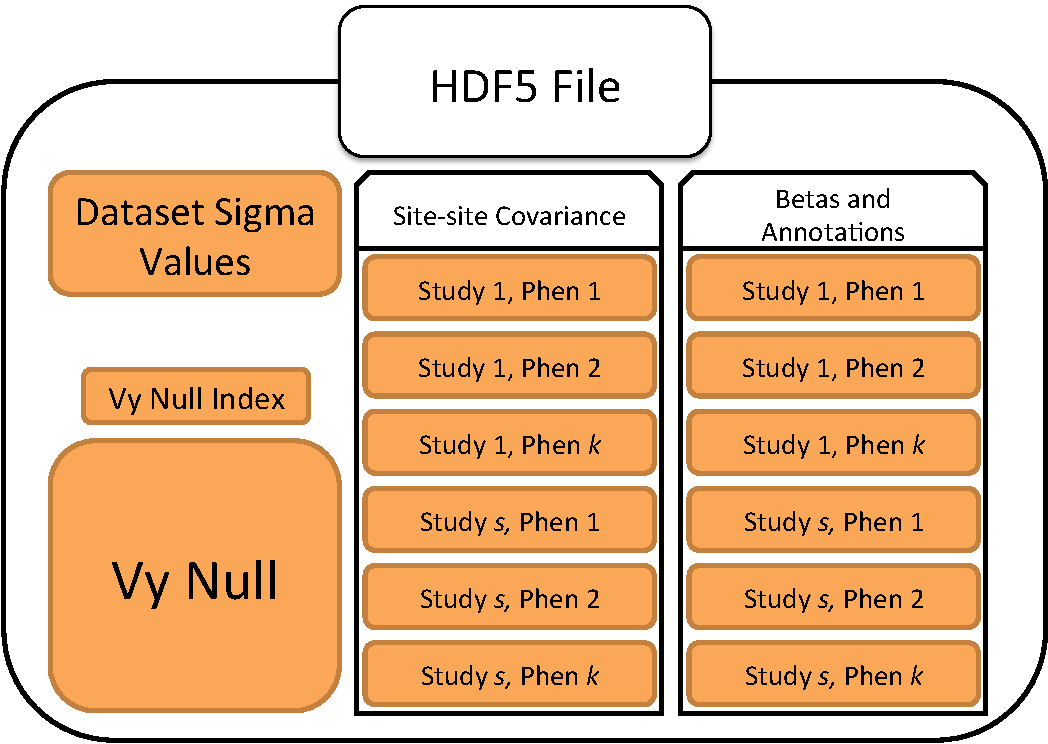
\includegraphics[width=\textwidth]{hdf5MAMBAMRP.pdf}
  \caption{Our HDF5 implementation contained the following components: first, a group with one table per annotation file. All effect size (beta) values and study-specific annotations were contained here, and the number of tables is limited by $S\ \textrm{(the number of studies)} \times K\ \textrm{(the number of traits)}$. Second, a group with site-site covariance data. While these covariance matrices may have dimension $M\ \textrm{(the number of variants)} \times M$, we store the data as tables, each row specifiying the covariance between two variants. The number of tables should be the same as the previous set, capped by $S\ \textrm{(the number of studies)} \times K\ \textrm{(the number of traits)}$. Third, we store one table with sigma values for each study/phenotype combination. In the event that the traits were rank-normal transformation was performed these sigma values are equal to 1. These are used to compute correlation between two datasets. Finally, we store a matrix/table pair for Vy null and its index. The Vy null matrix has dimensions $ (S \times K) \times (S \times K)$ each entry specifying the estimated correlation of effect sizes between two datasets. The index table encodes row/column position of each dataset.}
  \label{hdf5}
\end{figure}

 


\newpage

\bibliography{references}


\end{document}
